\section{PoP Part}
\label{sec:pop_part}
The Proof-of-Personhood is the part where most of the work has been focused. Some core features changed, as well as auxiliary functionalities that allows user to spare some useless (repeated) configurations. The major changes will be described in this section. Some minor improvements were also done, such as verifying if the conode was already linked before asking for the PIN.
\subsection{Multiple parties support}
\label{subsec:pop_mult_parties}
As stated previously, CP-MAC formerly handled only one party at the time. This limitation has been removed, and a user can now create, join or delete parties. 
\subsubsection{Implementation}
The singleton object that was taking care of all the party management operations has been converted to a simple object, where each party is now stored in his own directory. On creation, each party gets attributed a unique identifier with UUIDv4\footnote{\url{https://en.wikipedia.org/wiki/Universally_unique_identifier#Version_4_(random)}} format. The directory in which the party is stored is named after this identifier. The general directory structure now looks as follows :

\begin{center}
\begin{minipage}[c]{0.5\textwidth}
\dirtree{%
	.1 pop.
	.2 org.
	.3 RANDOM\_UUID\_1.
	.4 attendees.json.
	.4 conode.json.
	.4 description.json.
	.4 hash.json.
	.3 RANDOM\_UUID\_2.
	.4 ....
}
\end{minipage}
\end{center}

The use of this structure allows CP-MAC to just iterate over the entries of the \url{org} directory to lists the parties, which can be elegantly implemented in NativeScript as it provides interface to execute an action over each entry of a directory using a callback function. 

\subsubsection{Party statuses}
The PoP part of CP-MAC makes use of the status text abstractly described in section \ref{subsec:lists_ui} to show how the party is progressing across time. As these statuses aren't implemented in the Cothority back-end, here is a presentation of the different statuses and how they are deduced from the available data. Most of the statuses are inferred from the response of the \texttt{\textbf{FetchRequest}} message, that fetches the final statement from a conode :

\begin{description}
	\item[\textbf{\texttt{LOADING}}] is set until a response from the conode is received.
	\item[\textbf{\texttt{CONFIGURATION}}] is set when the returned message is a \texttt{"No config found"} error. It informs that the party is only stored locally, thus the conode don't have knowledge of it. 
	\item[\textbf{\texttt{PUBLISHED}}] is set when the returned message contains a final statement, but its list of attendees is empty. It informs that the party is stored on the conode, but not yet finalized.
	\item[\textbf{\texttt{FINALIZING}}] is set when the returned message contains a final statement, but its signature is empty. It informs that the instruction of finalizing has been given, but not on every conode.
	\item[\textbf{\texttt{FINALIZED}}] is set when the returned message contains a final statement, with a non-empty list of attendees and a signature. It informs that the instruction of finalizing has been given on every conodes.
	\item[\textbf{\texttt{ERROR}}] is set in the other cases. It informs that either the network is unavailable or an error occurred, thus the status of this party is unknown.
\end{description}

By using NativeScript primitive for time operations, the final statement can be regularly polled to give informative statuses to the user.

\subsection{Party proposals}
During the creation of a PoP-Party, its description must be shared through all the organizers. Until now, the chosen temporary solution was to use PasteBin, because the usual way of sharing information in CP-MAC (i.e using QR Code) don't have a sufficient capacity to store a party description. However, this had several drawbacks, such as depending on a third party service or giving public access to the party description.

A new procedure has been designed and works entirely on conodes. The general idea is that whenever an organizer publishes a party, the leader conode is used to propagate the description to the other conodes of the party. This way, the rest of the organizers can poll their conode and retrieve the description directly into CP-MAC. The configuration can then be opened in the standard party configuration page of CP-MAC, as seen on Figure \ref{fig:pop_config_ui} at page \pageref{fig:pop_config_ui}.

\begin{figure}[t]
	\centering
	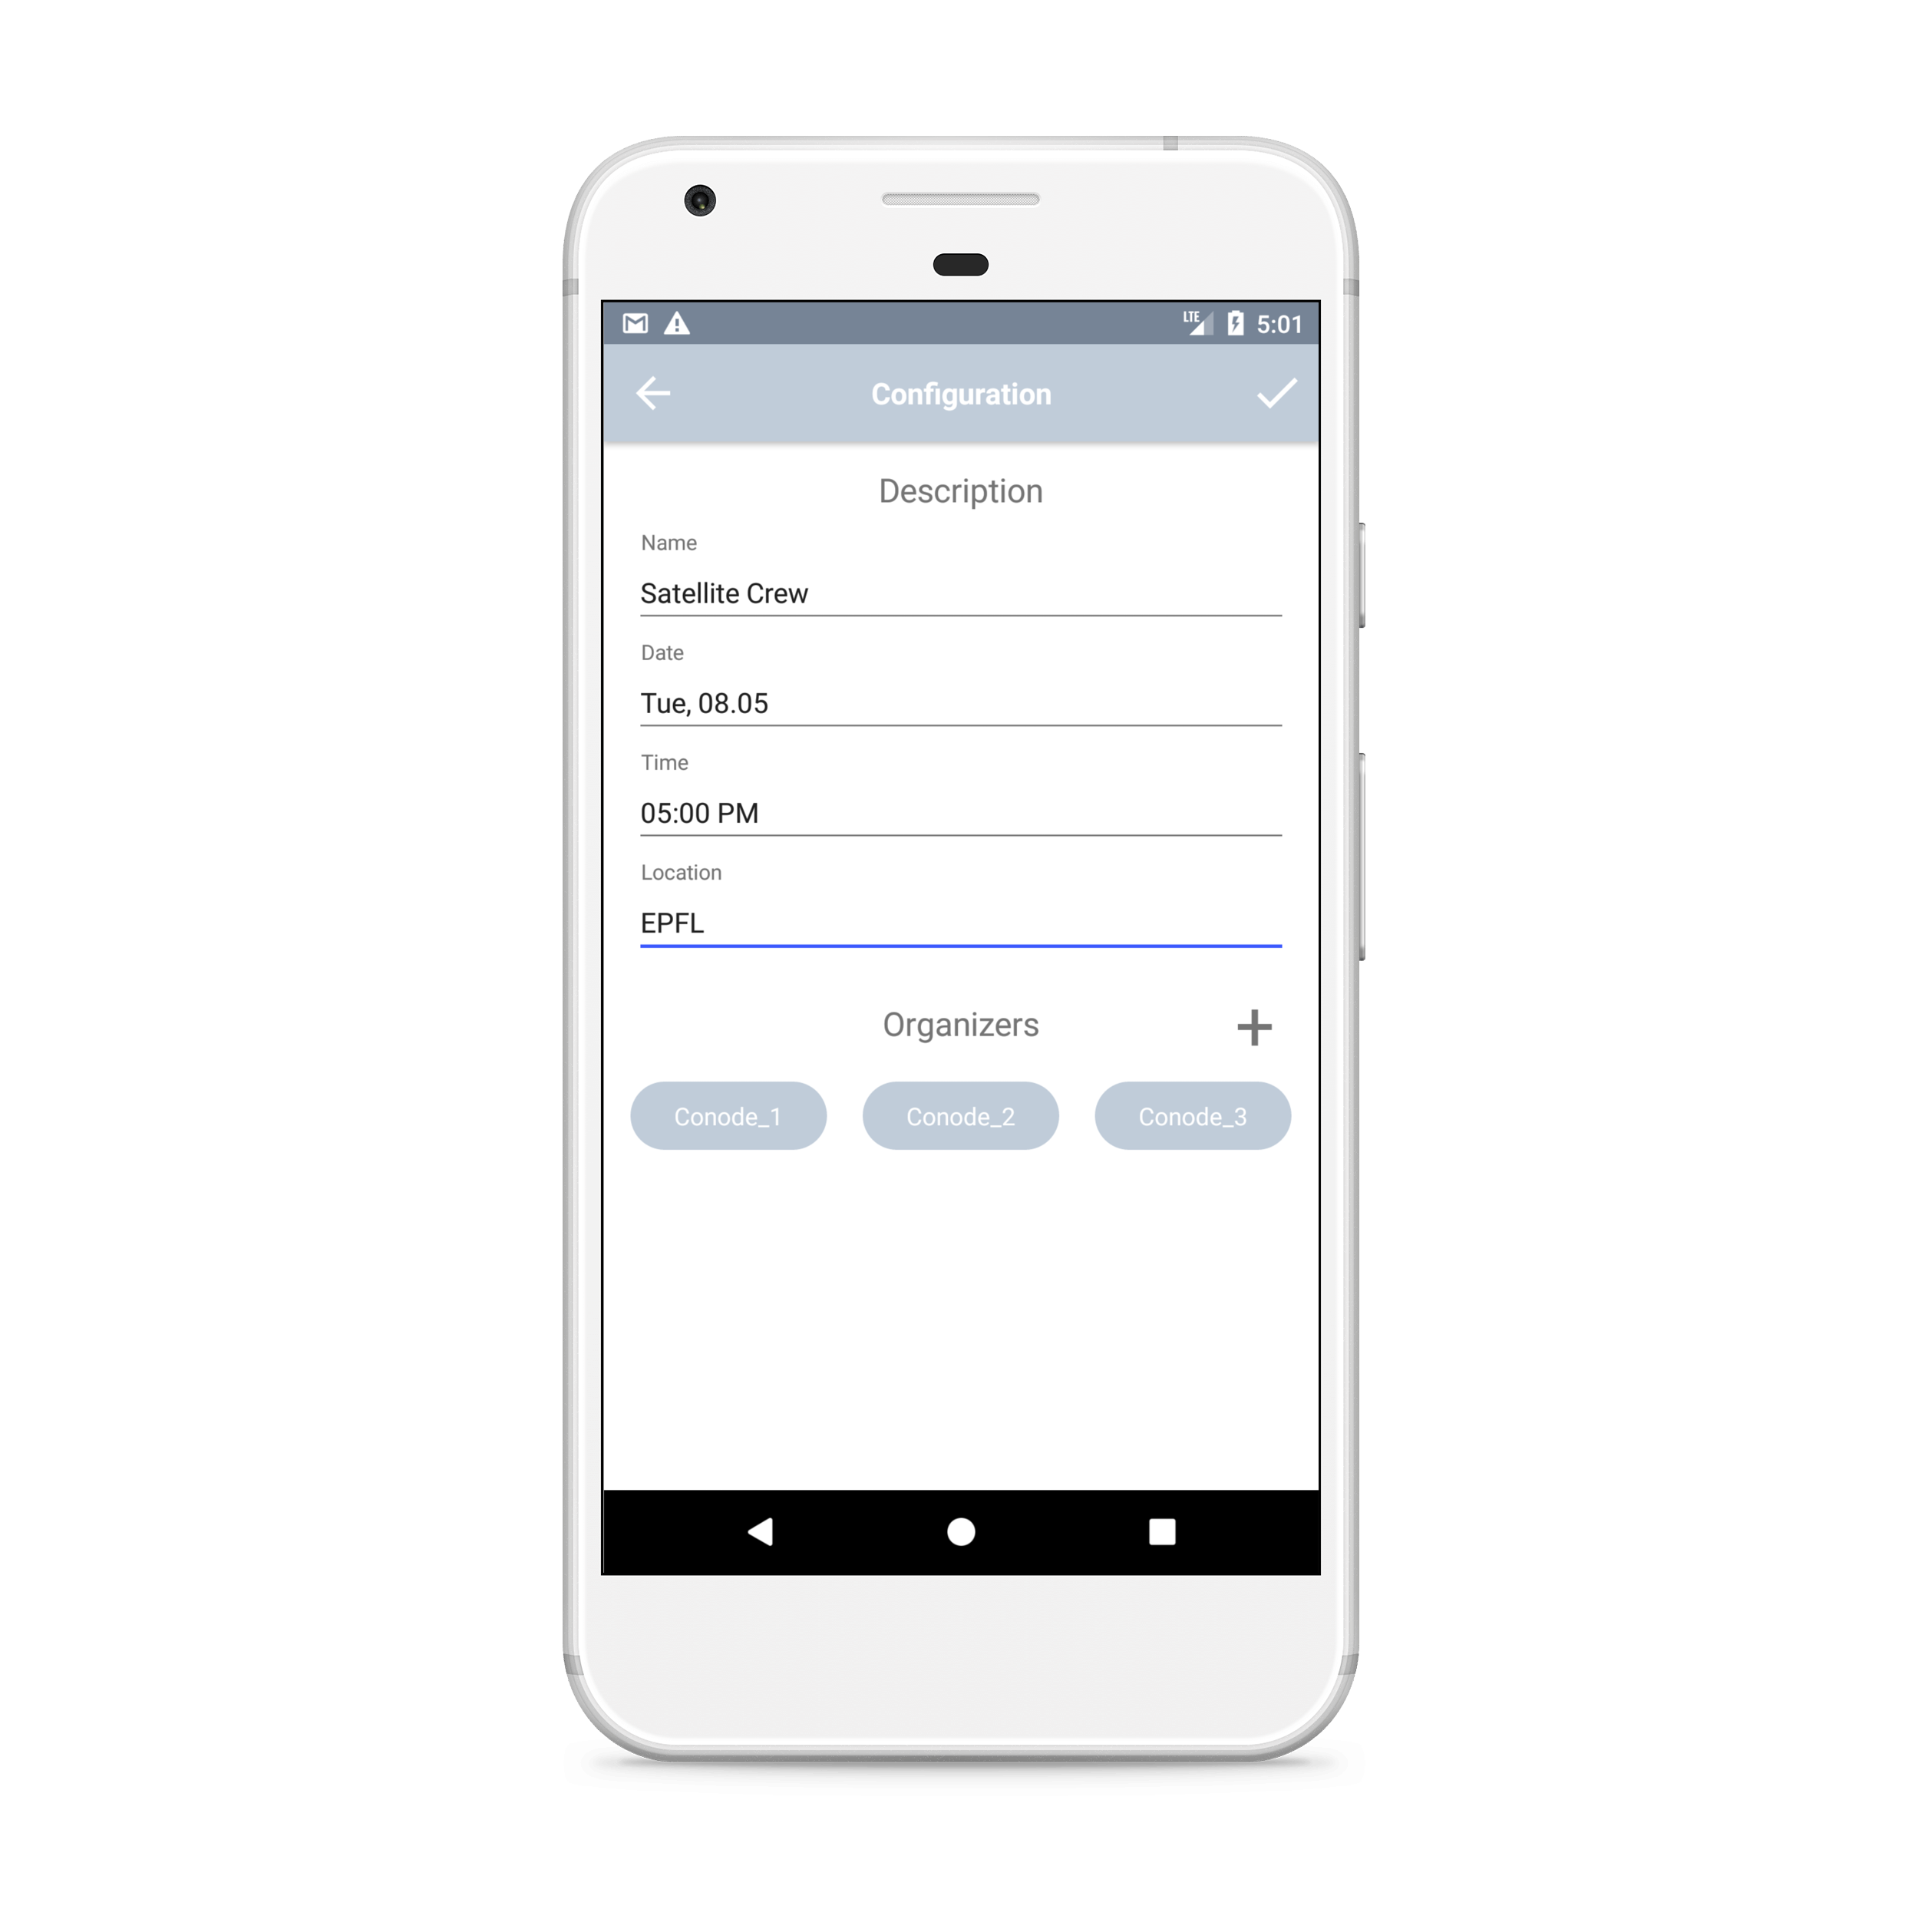
\includegraphics[height=0.8\linewidth]{resources/pop_config_ui.png}
	\caption{Example of a party configuration}
	\label{fig:pop_config_ui}
\end{figure}

\subsubsection{Implementation}
To achieve this, one message behavior has been updated in the Cothority back-end, and a new one has been added :
\begin{description}
	\item[StoreConfig] has been updated : besides storing a configuration on the conode, it will check if the conode is the leader one (i.e if it's the first one in the roster) and if so, it propagates the description to the rest of the roster. The conodes that receive the description will store it until it has been confirmed with \texttt{\textbf{StoreConfig}} within a maximum time period of one hour.
	\item[GetProposals] has been added: it retrieves every party proposals available on the conode.
\end{description}
\begin{figure}
	\centering
	\begin{tikzpicture}[->,>=stealth',shorten >=1pt,node distance=7cm,
scale = 0.6,transform shape, state/.style={circle, draw, minimum size=+75pt}]

\node[state] (Organizer 1) {\textit{Organizer 1}};
\node[state] (Conode 1) [right of=Organizer 1] {\textit{Conode 1}};
\node[state] (Organizer 2) [below of=Organizer 1, yshift=1.7cm] {\textit{Organizer 2}};
\node[state] (Conode 2) [right of=Organizer 2] {\textit{Conode 2}};

\path (Organizer 1) edge [bend left=35]              node [above] {1) \texttt{PinRequest}} (Conode 1)
(Organizer 1) edge [bend left=10]             node [above] {4) \texttt{StoreConfig}} (Conode 1)
(Organizer 1) edge [bend right=10]             node [below] {8) \texttt{Finalize}} (Conode 1)
(Organizer 1) edge [bend right=35]             node [below] {10) \texttt{FetchFinal}} (Conode 1)
(Organizer 2) edge             node [left]{2) QR Code \{Conode 2\}} (Organizer 1)
(Organizer 2) edge [bend left=35]              node [above] {1) \texttt{PinRequest}} (Conode 2)
(Organizer 2) edge [bend left=10]              node [above] {6) \texttt{GetProposals}} (Conode 2)
(Organizer 2) edge  [bend right=10]           node [below] {7) \texttt{StoreConfig}} (Conode 2)
(Organizer 2) edge [bend right=35]             node [below] {9) \texttt{Finalize}} (Conode 2)
(Conode 1) edge              node [right] {5) Party propagation} (Conode 2);

\end{tikzpicture}
	\caption{Graph of a party proposition and retrieval}
	\label{fig:proposal_graph}
\end{figure}
More specifically, here is the typical workflow that might happen for the complete creation of a party involving two organizers (Organizer 1 / Organizer 2) with their respective conode (Conode 1 / Conode 2). The numbers refer to the Figure \ref{fig:proposal_graph} at page \pageref{fig:proposal_graph}, where each link represents either an action or a message to the Cothority back-end.

\begin{enumerate}
	\item Each organizer authenticate to their respective conode
	\item \textit{Organizer 2} presents a QR Code containing his conode information, \{Conode 2\}
	\item \textit{Organizer 1} creates a new party and adds \textit{Organizer 2} to it by scanning the QR Code he is presenting
	\item \textit{Organizer 1} can then publish the party to his conode
	\item \textit{Conode 1} is the leader (first conode in the roster) so it propagates the party description to \textit{Conode 2}
	\item \textit{Organizer 2} can now retrieve the proposals list and notices a new entry
	\item  If the description of the party suits \textit{Organizer 2}, he can publish it to his conode
	\item When the party should end, \textit{Organizer 1} finalizes the party
	\item \textit{Organizer 2} also finalizes the party
	\item Any of the organizers can now fetch the final statement
\end{enumerate}
\subsubsection{Drawbacks and future work}
However, some drawbacks still remain. For example, if an organizer decides to change the description of the party, he has to start over and publish a new party.  This isn't convenient, as this require more time for the organizer than just editing the fields he wants to modify. Also, the other organizers will see a second entry when retrieving the proposals from their conode, which can be confusing and is more error-prone. Additionally, in the current schema, only one organizer decides of the details of the party, and the others only have the choice to accept (publish the party) or refuse (ignore) the current proposition. Again, a better procedure would allow any organizer to propose changes to the party description and when everybody agrees, they could publish it.

A solution to this problem could reside in the Cothorithy Cisc Identity Skipchains. Indeed, Cisc allows users to share key/value data using a private blockchain, on which any member can propose changes and cryptographically vote to accept or refuse changes. A threshold can also be set to define the minimum number of participant who should accept the changes to effectively add them to the blockchain. This would perfectly suit our requirements: each organizer could propose changes that will be reviewed by the rest and when everybody agrees on a description, they can publish it to their conode.
\subsection{Attendee part}
CP-MAC now supports a completely independent section for the management of attendee parties: a user can add a party by scanning the QR Code on the organizer's CP-MAC instance and benefits from the same status monitoring the organizers have. To keep things consistent in the code logic, a new base class \textbf{Party} has been extracted from the common traits of an attendee's party and an organizer's party. Each part can then have their respective \textbf{AttParty} and \textbf{OrgParty}, inherited from the base class.

The implementation of the \textbf{AttParty} will not be described here, as its implementation follows the \textbf{OrgParty} class (multiple parties support, directory structure, status retrieval). The only feature specific to the attendees is the way token are handled.
\subsubsection*{PoP-Token signature}
In contrast to the organizers, attendees make use of the PoP-Tokens, thus, when a party is finalized, the user can choose to generate his PoP-Token. CP-MAC handles the conversion from the final statement to the PoP-Token and makes it available to the user with all the other ones gathered through the previous parties. 

This list of PoP-Tokens will now be useful to the users as it is henceforth possible to sign arbitrary data transmitted using a QR Code and present the resulting signature (with the optional tag) via the same medium. Signatures are generated using (linkable) ring signatures, as described in section \ref{sec:linkable_ring_signature}.